
% \chapter{Background}
% \label{ch:Background}

% {\bf ARM TrustZone}~\cite{trustzone} is a widely available hardware-based TEE
% (Trusted Execution Environment) that partitions a device's CPU, memory, and
% peripherals, into two isolated logical ``worlds'' --- normal and secure. Each
% CPU core runs either in a non-secure state, where it has access only to
% resources assigned to the normal world, or a secure state where it has access to
% both normal and secure world resources. When switching between states (e.g., via
% the {\tt smc} instruction), the secure monitor, a critical and heavily-vetted
% software, is invoked to safely perform the transition. TrustZone enables a
% trusted OS to run in the secure world in conjunction with an OS in the normal
% world, and it protects state in the secure world even if the normal world is
% compromised.

% {\bf OP-TEE}~\cite{optee} is an open-source software stack that facilitates the
% use of ARM TrustZone. It provides a secure world OS (OP-TEE OS) for executing
% trusted applications; a low-level secure monitor for switching a core between
% non-secure and secure states; a TrustZone driver for normal world OSes such as
% Linux, which enables regular user-space applications to execute RPCs in the TEE;
% and a user-space supplicant that enables applications running in the TEE to
% access resources in the normal world OS.

\chapter{TrustZone \& OP-TEE Overview}
\label{ch:trustzone}

Trusted capsules allow advisory policies to be enforced on remote devices that the data owner does not
control. To protect sensitive operations such as trusted capsule policy evaluation
from remote users who can run an arbitrarily software stack, we require a \ac{TEE} 
that is resistant to potential compromise of both applications and \acs{OS} 
running on the remote device. 
We use
%Our trusted capsule data monitor uses 
ARM TrustZone technology as our \ac{TEE}
%to provide such a hardware-based trusted 
%execution environment (TEE)  
and Linaro OP-TEE as our \ac{TEE} low-level software stack.
%TrustZone software stack. 
Within this \ac{TEE}, we handle sensitive cryptographic operations, perform policy evaluation, 
securely store policy state, and anchor a secure channel to the policy coordinator. 

%In the following, we provide a brief overview of the properties of our TEE hardware TrustZone and 
%software stack Linaro OP-TEE. 

\section{TrustZone}

\textbf{ARM TrustZone}~\cite{trustzone} %provides a hardware-based TEE. It 
is widely available 
on current commodity ARM processors. TrustZone physically partitions the CPU, memory and peripherals 
into two isolated logical ``worlds'' -- normal and secure. 
Each world has its own banked system registers and MMU. 
To isolate the two worlds, all communications %between them 
must pass through a small and heavily verified  
\textit{secure monitor} gate. %, which executes at a privilege level higher than kernel code. 
To facilitate a 
\textit{world switch}, a special \textit{smc} instruction is used to trap into the secure monitor. 
The secure monitor saves the banked registers (e.g., return address, stack pointer) of the calling world 
and loads the banked registers of the callee world prior to executing \textit{eret} to return to the last 
execution point in the callee world. 

Where the \textit{smc} traps to is controlled by the secure world 
through its exception table register -- VBAR, which holds the memory address of the 
exception table. The memory that holds the exception table can also only be accessed by 
the secure world. 

The ARM TrustZone security model provides the following hardware-based guarantee: 
\textbf{the normal world cannot access the registers, memory or peripherals assigned 
to the secure world; but the secure world can access normal world registers and memory}. 

For registers, this guarantee is provided through a Secure-Modify-Only NS-bit in the ARM System 
Control Register (SCR), which controls the world-view for banked registers. Control of this bit is
retained exclusively by the secure world enabling it to access banked system registers
of both worlds, but not vice versa for the normal world. 

For memory, the secure world provides such a guarantee by either taking exclusive control of on-chip 
memory such as secure SRAM~\cite{hikey} or by mapping a section of the general off-chip memory and hiding it 
from the MMU of the normal world.

For peripherals, secure and normal world access are partitioned by interrupt modes. 
ARM processors contain two interrupt modes -- FIQ and IRQ. Each interrupt mode can be individually 
assigned to trap to code in the normal or secure world. Therefore, a peripheral can be
assigned to a specific world by assigning it to the corresponding interrupt mode. The usual set-up 
assigns FIQ to the secure world and IRQ to the normal world, as most existing normal world drivers 
currently operate using the IRQ mode.

For additional hardware protection for off-chip memory and device protection, additional hardware, 
such as TrustZone Protection Controller (TZPC) and TrustZone Address Space Controller (TZASC), can
be added to extend the dual-world abstraction to the AXI-bus, memory controllers and interrupt controllers.

\begin{table}
\begin{center}
\begin{tabular}{|l||*{2}{c|}}\hline
%\backslashbox{Privilege}{World}
&\makebox{Secure}&\makebox{Normal}\\\hline\hline
EL0 &Trusted Application&Application\\\hline
EL1 &Secure \ac{OS}&Normal \ac{OS}\\\hline
EL3 &Secure Monitor&-\\\hline
\end{tabular}
\caption{ARM processor modes.}
\label{Tbl-TrustZone}
\end{center} 
\end{table}

The secure/normal paradigm operates orthogonally to the traditional concept of privilege levels, see 
Table~\ref{Tbl-TrustZone}. The secure monitor operates in secure mode at the highest privilege level (EL3), 
while untrusted application code and privileged normal world \ac{OS} operate in non-secure mode. 
The secure mode at privilege level EL0 and EL1 is reserved for trusted applications and the 
trusted \ac{OS}. 

Architecturally, the privilege level of the CPU is controlled by a system register called 
Saved Program State Register (SPSR). The SPSR register is banked between different modes of operation
for the ARM processor and is saved/reloaded during a world switch  before returning to the point of last
execution. The current SPSR in use is loaded into the Current Program State Register (CPSR).

TrustZone enables the applications and the \ac{OS} running in the secure
World to remain protected even if the normal world \ac{OS} or applications
are arbitrarily compromised.

%It's security capabilities are similar to two 
%separate physical machines connected by a thin communication interface, but packaged more compactly as a 
%single-chip solution. 
%Alternatively, TrustZone can be replicated architecturally with two CPUs, 
%TrustZone's world abstraction has the advantages of requiring less on-chip space, 
%being more energy efficient and enabling symmetric processing. 

\section{Linaro OP-TEE}

\textbf{Linaro OP-TEE} is an open-source software stack for ARM
TrustZone. It provides a secure world \ac{OS} (OP-TEE OS) for executing
trusted applications, a low-level secure monitor for world-switching
(ARM Trusted Firmware) and a TrustZone driver (OP-TEE Linux driver \&
OP-TEE Supplicant) for the normal world \ac{OS}, such as Linux, to access
TrustZone and execute secure world RPCs. We use Linaro OP-TEE as-is except 
for our custom extensions that enable direct access to the network and the 
file system as RPCs by trusted applications in the secure world.
These secure world RPCs are executed by OP-TEE Supplicant which runs in 
normal world user space as a single threaded application and are intermediated 
by OP-TEE Linux Driver in the normal world kernel. 


The following description is based on the HiKey system-on-chip (SoC) with Linux as the normal world 
OS. 

\subsection{ARM Trusted Firmware}
\textbf{ARM Trusted Firmware (ATF)}~\cite{atf} is a set of reference boot and runtime firmware designs for 
ARM TrustZone. It initializes the secure world through a multi-staged boot sequence, as shown in
Figure~\ref{fig:bootsequence}. 
A root-of-trust can be built by having each stage attest the image of the 
next. 

%In ATF, transition between boot stages is controlled by several key global data structures:

%\begin{itemize}
%\item  \textit{entry\_point\_info} -- controls the privilege level of the CPU after executing 
%\textit{eret} or \textit{smc}
%\item  \textit{image\_info } -- image size of each boot stage
%\item  \textit{mem\_info\_t} -- available secure SRAM
%\item  \textit{bl31\_params} -- stores information about the secure and normal world OS images 
%for the secure monitor
%\end{itemize}

%%%%%%%%%%%%%%%%%%%%
\begin{figure}
\centering
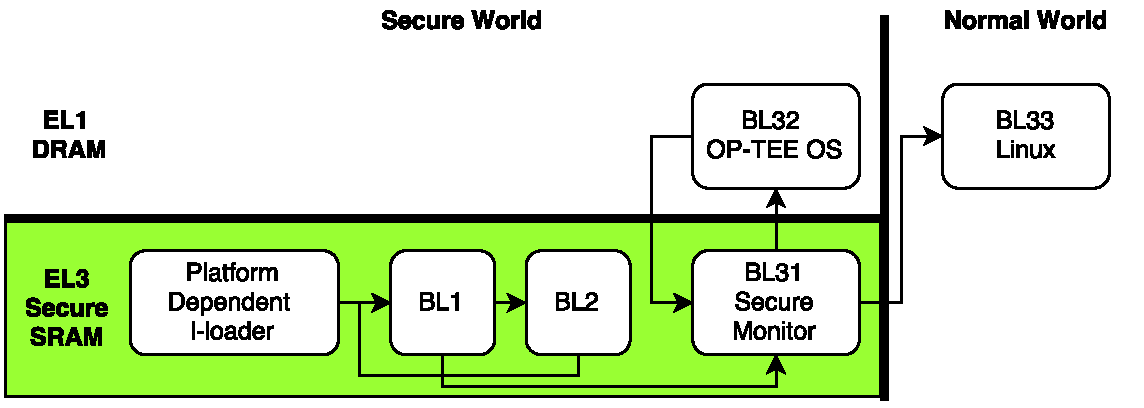
\includegraphics[width=\columnwidth]{fig/bootsequence.pdf}  
\caption{ARM TrustZone Boot Sequence.}
\label{fig:bootsequence}
\end{figure}
%%%%%%%%%%%%%%%%%%%%	

%The first stage consists of two components: a platform dependent (e.g., HiKey) l-loader~\cite{lloader} 
%and the first stage of ATF boot (BL1). When the processor resets, it begins execution in Secure EL3 mode. 
%It jumps to a pre-set address in secure SRAM where a HiKey loader program (l-loader) redirects execution to 
%the ATF's first stage boot sequence. The first stage boot sequence sets up the EL3 runtime environment with
%the following sequence of actions:

%\begin{enumerate}
%\item  Initializes the exception vector table VBAR\_EL3
%\item  Initialize console and timer
%\item  Create EL3 MMU page table mappings for BL1 image
%\item  Load, verify and execute BL2 image in SRAM
%\end{enumerate}

%The second stage (BL2) sets up the EL1 runtime environment through a similar sequence of actions:

%\begin{enumerate}
%\item  Initializes the exception vector table VBAR\_EL1
%\item  Configure SRAM and CPU (e.g., clock rate, frequency dividers etc,.)
%\item  Create EL1 MMU page table mappings for BL2 image
%\item  Load, and verify BL31, BL32, Bl33 images in SRAM
%\end{enumerate} It (1)

%The third stage (BL3) is further divided into three sub-stages: BL31, BL32, and BL33.

%The first sub-stage (BL31) is the secure monitor. To execute at EL3, BL2 jumps to BL31 using an 
%\textit{smc} exception. Execution flow is redirected to the exception table pointed to by VBAR\_EL3, 
%which was set up during BL1. It is the last boot stage that executes in secure SRAM. It performs the 
%following sequence of actions:

%\begin{enumerate}
%\item  Re-initialize the exception vector table VBAR\_EL3 to a new runtime exception table
%\item  Initialize a \textit{cpu\_data\_t} structure per CPU to store pointers to the CPU's secure
% (\textit{opteed\_context\_t}) and non-secure contexts (\textit{cpu\_context\_t})
%\item  Allocate a C runtime stack for each CPU to use
%\item  Create EL3 MMU page table mappings for BL31 secure monitor image
%\item  Initialize the general interrupt controller (GIC), DMA, power control and real-time clock
%\item  Set up OP-TEE OS (EL1) entry-points and initialize secure CPU contexts
%\end{enumerate}

%The second sub-stage (BL32) contains the secure OP-TEE OS and runs at EL1 in the secure world. Currently, 
%ATF supports both OP-TEE OS and NVIDIA TLK~\cite{tlk}, although only OP-TEE OS seem to be actively 
%supported. The initialization procedure for the secure OS is rather complicated but involve the following 
%key steps:

%\begin{enumerate}
%\item Map a portion of unsecure DRAM (e.g., Hikey board -- 16MB) for OP-TEE OS
%\item Initialize each CPU with a secure context
%\item Re-initialize VBAR\_EL1 register to point to the same exception table pointed to by VBAR\_EL3
%\item Return a \textit{thread\_vector\_table} to the secure monitor that specifies entry-points 
%into OP-TEE OS
%\end{enumerate}

%The entry-points are stored by the secure monitor's handler (e.g., \textit{opteed\_smc\_handler}). 
%The handler operates as a state machine that controls all transitions between OP-TEE OS and normal world OS. 
%If the calling world is normal world, it performs the context switch to the secure world, and vice versa. 
%If also handles transitions due to RPC, interrupts and the initial boot process. The handler also initializes 
%and sets up the \textit{intr\_type\_desc}, which controls the interrupt routing model. The interrupt routing
%model specifies the destination world for IRQ and FIQ exceptions. The availability of these interrupts can be 
%masked by control bits in the SPSR registers.

%Once OP-TEE OS is initialized and returns to the secure monitor, the secure monitor then loads and boots 
%the normal world OS (Bl33). The third sub-stage (BL33) contains the normal world OS (Linux) and its 
%bootloader (EUFI/GRUB). This is the first stage that executes in the normal world. The boot sequence from 
%this point on is as-is for systems without TrustZone.

%Context switching between secure (BL32) and normal world (BL33) is handled by the secure monitor 
%(BL31). For each processor mode in~\ref{Tbl-TrustZone}, there are two stack pointers: one
%mode-specific stack pointer SP\_ELn and one general purpose stack pointer SP\_EL0. SP\_EL0 is 
%saved on context switches, while the mode-specific SP\_ELn is used to store the location of the 
%saved context. A context consists of all the EL3 and EL1 system registers,and all general purpose 
%registers (x0-x29, SP\_EL0, lr). The full list of relevant registers is defined with the
%\textit{DEFINE\_REG\_STRUCT} macro in the source code. When switching contexts, the secure monitor 
%controls the destination privilege level, interrupt masks and security state by modifying the NS-bit 
%in SCR and the interrupt mask and mode bits in SPSR.

\subsection{OP-TEE OS} 
 
\textbf{OP-TEE OS} is capable of multi-threading, memory management, and
running and isolating trusted applications. OP-TEE OS does not have a scheduler. It operates as a 
slave in a master-slave relationship with the normal world OS. Therefore, OP-TEE OS can only 
simultaneously run as many trusted application instances as there are cores at any given time. 
On multi-core architectures, each CPU can independently perform a world switch. When an interrupt
occurs that needs to be handled by the normal world, OP-TEE OS transitions back into the
normal world and once the interrupt has being handled, returns to its last point of execution within 
the secure world. Communication between the normal world and secure world occurs through a piece of 
pre-allocated shared memory accessible by both worlds. The shared memory is allocated by 
the secure world but is managed by the normal world. The secure world OS may access peripherals 
under the normal world's control and allocate shared memory through RPC calls into the normal world. 
For example, OP-TEE OS uses these RPC calls to access the normal world file system, with which it 
implements secure storage using a provisioned root key. 

OP-TEE OS provides useful abstractions to build trusted applications that run in secure world 
user space (Secure EL0). Trusted applications can be single-instance or multi-session. 
OP-TEE OS applications conform to the GlobalPlatform Internal API~\cite{globalplatformAPI} where 
each trusted application must implement a set of well-defined functions as entry-points. Client 
applications in the normal world invoke these functions through a similar set of GlobalPlatform 
Client API~\cite{globalplatformAPI}. The list of functions are listed in 
Table~\ref{Tbl-GlobalPlatformAPI}. We use these APIs and secure storage provided by OP-TEE OS to build 
our multi-session trusted capsule application at the core of our trusted capsule monitor. Any call into 
trusted applications from the normal world are serialized on the normal world side by the TrustZone 
device driver.   

%\begin{adjustwidth}{-0.75in}{-0.75in}
%\noindent\makebox[\textwidth]{%
\begin{table*}[t]
\small
\begin{center}
\begin{tabular}{ |p{0.3\textwidth}|p{0.25\textwidth}|p{0.35\textwidth}| } 
 \hline
 \textbf{Internal API} & \textbf{Client API} & 
\textbf{Function} \\\hline\hline 
 CreateEntryPoint & InitializeContext & Initialize a context in TrustZone driver \\\hline
 DestroyEntryPoint & FinalizeContext & Deletes a TrustZone context\\\hline
 OpenSessionEntryPoint & OpenSession & Creates an instance of the 
trusted application \\\hline
 CloseSessionEntryPoint & CloseSession & Destroys an instance of the 
trusted application \\\hline
 InvokeCommandEntryPoint & InvokeCommand & Call one of trusted 
application's functions \\\hline
 - & RegisterSharedMemory & Registers a chunk of memory for use between 
the two worlds\\\hline
 - & AllocateSharedMemory & Allocate a chunk of memory from the shared 
memory pool\\\hline
 - & ReleaseSharedMemory & Free a chunk of memory allocated from the 
shared memory pool\\\hline
 - & RequestCancellation & Request an instance of trusted application to 
stop and return\\\hline
\end{tabular}
\caption[Linaro OP-TEE API.]{Linaro OP-TEE API. Internal APIs are used by trusted applications 
and are prefixed by \textit{TA\_}. Client APIs are used by the normal world and are prefixed 
by \textit{TEEC\_}.} 
\label{Tbl-GlobalPlatformAPI}
\end{center}
\end{table*}
%}
%\end{adjustwidth}

\subsection{OP-TEE Linux Driver}

\textbf{OP-TEE Linux Driver} provides the normal world \ac{OS} (Linux) access to TrustZone. 
It represents TrustZone as a device file, which can be accessed from the normal world through 
the set of APIs listed in Table~\ref{Tbl-GlobalPlatformAPI} from both user and kernel space. 
The TrustZone driver is responsible for two main tasks -- (1) calling into trusted applications 
running in TrustZone and (2) handling RPC requests from OP-TEE OS (e.g., file system, shared memory 
allocations). For trusted capsules, we extended the limited set of RPC calls available to the 
OP-TEE OS to include networking and direct file system operations. The TrustZone driver executes 
RPCs by using the OP-TEE Supplicant. 

When the TrustZone driver calls into the secure world, it uses two unique identifiers -- "session 
object" and "function ID". Each trusted application instance is represented by a "session" and each 
function that the trusted application can perform by a "function ID". Together, these two identifiers 
specify the entry point for the call into secure world. Function parameters are passed by value or by 
reference through shared memory between the two worlds. 

%Shared memory can either be allocated and re-used by the normal world application or it can be temporary, in 
%which case the allocation and de-allocation occurs transparently. In both cases, moving data from client 
%buffers require a copy to and from the shared memory between the two worlds. 

\subsection{OP-TEE Supplicant}

\textbf{OP-TEE Supplicant} takes RPC invocations from OP-TEE Linux Driver and executes the equivalent 
system calls through the normal world OS to access the relevant peripheral devices. These peripheral 
devices can include file system block devices and network cards for I/O. 
Linux \textit{dmabuf} and \textit{mmap} are used to pass data between the user space
OP-TEE supplicant and kernel space OP-TEE Linux Driver. 
Only a single instance of the OP-TEE supplicant 
can run at any given time and this is enforced by the OP-TEE Linux Driver. We do not intercept any 
systems calls made by the OP-TEE Supplicant running in normal world user space. 
%This does not affect the 
%advisory policy enforcement or the confidentiality and integrity guarantees of trusted capsules. 
The OP-TEE Supplicant never accesses decrypted trusted capsule data and it
cannot write to a capsule without the corruption being detected.  